%!TEX TS-program = xelatex

% -- Document Class -----------------------------------------------------------

\documentclass[a4paper, 12pt]{article}

% -- Packages -----------------------------------------------------------------

% Language
\usepackage{polyglossia}
	\setmainlanguage{german}
	\setotherlanguage{english}
% Citations
\usepackage[style=alphabetic, backend=biber]{biblatex}
	\addbibresource{References.bib}
% Caption support
\usepackage{caption}
% Context sensitive quotation
\usepackage{csquotes}
% Customized enumeration
\usepackage{enumerate}
% Extend options for positioning floats
\usepackage{float}
% Support highlighting of certain parts of the text
\usepackage{framed}
% Include graphics
\usepackage{graphicx}
% Defines the number of the last page in the document
\usepackage{lastpage}
% Tools for mathematical typesetting
\usepackage{mathtools}
% For code sections
\usepackage{moreverb}
% Headings
\usepackage[automark, nouppercase]{scrpage2}
% To change the format of titles
\usepackage{titlesec}
% Support for unicode math fonts
\usepackage{unicode-math}
% Color support
\usepackage[x11names]{xcolor}
% Extras for XƎTEX
\usepackage{xltxtra}
% Hyperlinks and pdf properties
\usepackage{hyperref}

% -- Fonts --------------------------------------------------------------------

% Use same size for numbers and other text
\defaultfontfeatures{Numbers=Lining}

% Set fonts for document
\setmainfont[Mapping=tex-text]{Avenir Next}
\setsansfont[Mapping=tex-text]{Ubuntu}
\setmonofont[Scale=MatchLowercase]{Menlo}
\setmathfont{Asana-Math.otf}

% Define font styles
\newfontfamily\Zapfino{Zapfino}

% -- Macros -------------------------------------------------------------------

\newcommand{\Title}{Hilfsunterlagen}
\newcommand{\TitleDescription}{Algorithmen Und Datenstrukturen}
\newcommand{\Version}{8}
\newcommand{\Subject}{Diverse Unterlagen zur LVA Algorithmen und Datenstrukturen}
\newcommand{\Location}{Wien}
\newcommand{\Keywords}
{
	Algorithmen und Datenstrukturen 1,
	Dynamische Programmierung,
	Hashfunktionen,
	Laufzeitbestimmung,
	Matrix
}
\newcommand{\LeftFooter}{Algodat-Hilfsunterlagen}

\newcommand{\AuthorOne}{-}
\newcommand{\MailOne}{\href{mailto:sanssecours@f-m.fm}{sanssecours@f-m.fm}}

\newcommand{\codeinput}[1]
{
    \begin{leftbar}
        \input{Code/#1}
    \end{leftbar}
}

% -- Colors -------------------------------------------------------------------

% Background color for syntax highlighting
\definecolor{bgcolor}{rgb}      {1,     1,      1}

% Custom color definitions
\definecolor{aqua}{rgb}         {0,     0.56,   1}
\definecolor{bluegray}{rgb}     {0.22,  0.46,   0.84}
\definecolor{grape}{rgb}        {0.56,  0,      1}
\definecolor{orchid}{rgb}       {0.41,  0.13,   0.55}
\definecolor{orange}{rgb}       {1,     0.54,   0}
\definecolor{silver}{rgb}       {0.57,  0.57,   0.57}
\definecolor{turquoise}{rgb}    {0,     0.86,   0.84}

% -- Syntax Highlithing -------------------------------------------------------

% Syntax highlighting definitions
% Text
\newcommand{\hlstd}[1]{\textcolor{black}{#1}}
% Numbers
\newcommand{\hlnum}[1]{\textcolor{DarkOrchid4}{#1}}
\newcommand{\hlesc}[1]{\textcolor[rgb]{1,0,1}{#1}}
% Strings
\newcommand{\hlstr}[1]{\textcolor{SeaGreen3}{#1}}
\newcommand{\hlpps}[1]{\textcolor[rgb]{0.51,0.51,0}{#1}}
\newcommand{\hlslc}[1]{\textcolor[rgb]{0.51,0.51,0.51}{\it{#1}}}
\newcommand{\hlcom}[1]{\textcolor{aqua}{#1}}
\newcommand{\hlppc}[1]{\textcolor[rgb]{0,0.51,0}{#1}}
\newcommand{\hlopt}[1]{\textcolor[rgb]{0,0,0}{#1}}
\newcommand{\hllin}[1]{\textcolor[rgb]{0.33,0.33,0.33}{#1}}
% Keywords
\newcommand{\hlkwa}[1]{\textcolor{DodgerBlue3}{#1}}
\newcommand{\hlkwb}[1]{\textcolor[rgb]{0,0.34,0.68}{#1}}
\newcommand{\hlkwc}[1]{\textcolor{DarkOrchid4}{#1}}
% Functions
\newcommand{\hlkwd}[1]{\textcolor{orange}{#1}}

% -- Document Properties ------------------------------------------------------

\setlength\parindent{0cm}

\hypersetup
{
	pdftitle	= {\Title},
	pdfsubject	= {\Subject},
	pdfauthor	= {\AuthorOne},
	pdfkeywords = {\Keywords},
	colorlinks	= true,
	linkcolor	= black,
	anchorcolor = black,
	citecolor	= silver,
	urlcolor	= orange
}

% -- Header and Footer --------------------------------------------------------

\clearscrheadings
\renewcommand{\headfont}{\normalfont}
\ihead{\headmark}
\ohead{}
\ifoot{\LeftFooter}
\ofoot{\thepage/\pageref{LastPage}}

\setlength{\headheight}{1.8\baselineskip}
\setheadsepline{0.5pt}
\setfootsepline{0.5pt}

% -- Titlepage ----------------------------------------------------------------

\pagestyle{empty}
\begin{document}

\begin{titlepage}
    \begin{center}
        % Title and title-description
        {\Huge\Zapfino\Title}
        \vskip 0.5cm
        {\color{aqua}\hrule}
        \vskip 0.5cm
        {\Large\textit\TitleDescription}
        \vskip 14cm
    \end{center}

    % Date and version number
    \begin{leftbar}
        \begin{tabular}{ll}
            \textbf{Kontakt}    & \MailOne\\
            \textbf{Version}    & \Version\\
            \textbf{Datum}      & \today
        \end{tabular}
    \end{leftbar}

\end{titlepage}


% -- Table of Contents --------------------------------------------------------

% Set section format for table of contents
\titleformat{\section}{\sffamily\bfseries}{}{0pt}{}[{\color{aqua}\hrule}]

\makeatletter \renewcommand{\@dotsep}{10000} \makeatother
\newpage
\setcounter{page}{2}
\tableofcontents

% -- Section & Paragraph Style ------------------------------------------------

% Set format for section
\titleformat{\section}
    {\large\sffamily\bfseries}  % Large, bold, sans serif font for section
    {}                          % No format applied to whole title
    {0pt}                       % No separation between label and title
    {\thesection~·~}            % Start with section number
    [{\color{aqua}\hrule}]      % Underline with blue ruler

% Set format for other sections and paragraphs
% Color = orchid, Font = bold, sans serif
\titleformat*{\subsection}{\color{orchid}\sffamily\bfseries}
\titleformat*{\subsubsection}{\color{orchid}\sffamily\bfseries}
\titleformat*{\paragraph}{\color{orchid}\sffamily\bfseries}
\titleformat*{\subparagraph}{\color{orchid}\sffamily\bfseries}

% -- Page Style ---------------------------------------------------------------

\newpage
\pagestyle{scrheadings}

%-- Text ----------------------------------------------------------------------

\begin{abstract}

	\noindent Dieser Text ist mit der Absicht entstanden zu helfen. Ich habe
    ihn somit natürlich nicht aus Absicht mit Fehlern gespickt. Trotzdem ist
    es doch sehr wahrscheinlich, dass er Fehler enthält. Ich bitte das zu
    entschuldigen, und möchte damit den Hinweis geben, dass für jeglichen
    Inhalt dieses Textes \emph{absolut kein Gewähr auf Richtigkeit} gegeben
    wird.\\

	\noindent Solltet ihr Fehler im Text finden wäre es sehr nett wenn ihr mir
    eine \href{mailto:sanssecours@f-m.fm}{e-Mail} schreibt, damit ich sie
    ausbessern kann.

\end{abstract}

\section{Laufzeiten}

\subsection{Beweisen oder Widerlegen des asymptotischen Wachstums von
Funktionen}

\subsubsection{Umformung}

Der erste Schritt am Anfang der Analyse einer Funktion wie z.B.

\begin{equation}
	\label{function:Laufzeit}
	f(n) = \left\{
	\begin{array}{l l}
		2⋅ n² + \frac{n²}{2} + 10 & \text{wenn $n < 50$}\\

		0.5 ⋅ n^\frac{1}{2}       & \text{wenn $n$ ungerade und $n ≥ 50$}\\

		\frac{1}{2}⋅ n + \frac{n²}{n} ⋅ \log\left(n²\right) - \frac{1}{10}
                                  & \text{sonst}
	\end{array} \right.
\end{equation}

besteht darin zu bestimmen welche Teile der Funktion für unendlich viele $n$
gelten und welche Glieder wiederum ab eine bestimmten $n$ nicht mehr
vorkommen, also nur für endlich viele $n$ gelten.\\

In Funktion \ref{function:Laufzeit} kann man den ersten Zweig vernachlässigen
da er ab $n ≥ 50$ nicht mehr gilt. Damit man diesen Teil auch wirklich nicht
beachten muss ist $n₀$ auf einen Wert $≥ 50$ zu setzen. Der nächste Schritt
besteht darin die Funktion ein wenig zu vereinfachen. Dazu einmal ein paar
einfache mathematische Umformungen die hier recht nützlich sind:

\[
	a^{\frac{1}{b}} = \sqrt[b] a	\quad~
	a^{-b} = \frac{1}{a^b}			\quad~
	\frac{a^b}{a^c} = a^{b-c}		\quad~
	a^b ⋅ a^c = a^{b+c}				\quad~
	\log\left(a^b\right) = b⋅ \log\left(a\right)
\]

Nach der Umformung der Funktion ohne den ersten Zweig, den wir ohnehin für den
Beweis/Widerlegung vernachlässigen wollen bekommen wir:

\begin{figure}[H]
		\caption{Vereinfachte Funktion für $n≥50$}
		\label{figure:Vereinfachte_Funktion}
\[
	f(n) = \left\{
	\begin{array}{l l}
		0.5⋅ \sqrt n        & \text{wenn $n$ ungerade}\\
		\frac{1}{2}⋅ n + 2 n ⋅ \log\left(n\right) - \frac{1}{10}
                            & \quad \text{sonst}
	\end{array} \right.
\]
\end{figure}

\subsubsection{Vereinfachte Terme mit asymptotisch gleicher Laufzeit in Theta-Notation}

Als nächsten Schritt könne wir jetzt Terme für die Zweige unserer Funktionen
bestimmen die die „gleiche” Laufzeit wie die Terme unserer ursprünglichen
Funktion besitzen. Das ist vor allem praktisch wenn wir angeben wollen wie die
unteren und oberen Schranken unserer Funktion aussehen. Dazu bestimmen wir in
jedem Zweig den „größten” und somit den für die Laufzeit bestimmenden Teil.\\

In der zweiten Zweig unserer Funktion ist der bestimmende Teil der Term $\sqrt
n$. Die Konstante können wir streichen, da sie nichts am asymptotischen
Wachstum der Funktion ändert.\\

Im dritten Zweig könne wir erkennen, dass „$2 n ⋅ \log n$” den für das
Wachstum wichtigen Teil darstellt. Die Konstante spielt keine Rolle für das
Wachstum. Somit kommen wir hier auf den Term „$n \log n$” der asymptotisch
gleiches Wachstum wie unsere Ausgangsterm aufweist. Die gesamte vereinfachte
Funktion, die für ein $n≥ 50$ das gleiche Wachstum wie die Ausgangsfunktion
aufweist ist in Abbildung \ref{Figure:Vereinfachte_Funktion_Gleiches_Wachstum}
zu sehen.

\begin{figure}[H]
	\caption{Funktion mit asymptotisch gleichem Wachstum wie die
	Ausgangsfunktion ab $n≥50$}
	\label{Figure:Vereinfachte_Funktion_Gleiches_Wachstum}
\[
	\label{function:Laufzeit_Vereinfacht}
	f(n) = \left\{
	\begin{array}{l l}
		\sqrt n     & \quad \text{wenn $n$ ungerade}\\
		n \log n    & \quad \text{sonst}
	\end{array} \right.
\]
\end{figure}

Aus der vereinfachte Funktion können wir gleich erkennen, dass alle Funktionen
die eine Laufzeit in $θ\left(n \log n\right)$ besitzen oder schneller wachsen
eine obere Schranke für unsere Funktion darstellen. Alle Funktionen die eine
Laufzeit in $θ\left( \sqrt n\right)$ aufweisen oder langsamer wachsen stellen
eine untere Schranke dar. Die Funktion $g\left(n\right)=n$ hingegen würde
weder eine untere noch eine obere Schranke darstellen, da sie zwar ein
schnelleres Wachstum als der erste Zweig unserer Funktion aufweist, aber eben
auch langsamer als der zweite Zweig wächst.

\subsubsection{Beweis}

Wir wollen nun beweisen, dass $\sqrt n$ eine untere Schranke für unsere
Funktion darstellt also $f\left(n\right) = Ω \left(\sqrt n\right)$ gilt. Dazu
schreiben wir als erstes laut Definition an:
\[
	f\left(n\right)=Ω \left(\sqrt n\right) \quad ⇒ \quad
	∃ c,n > 0 \quad ∀ n≥ n₀: 0 ≤ c ⋅ \sqrt n ≤ f\left(n\right)
\]

Wir müssen diese Bedingung nun für beide Zweige beweisen und passende Werte
für $c$ und $n₀$ finden, wobei wir von $n₀$ schon wissen, dass wir einen Wert
$≥ 50$ nehmen sollten, da wir ansonsten auch den ersten Zweig unserer Funktion
beachten müssten, der nur für $n < 50$ gilt. Wir sehen uns nun die beiden
anderen Zweige in der vereinfachten Form aus
Abbildung~\ref{figure:Vereinfachte_Funktion} an.

\[
	∃ c,n > 0 \quad ∀ n ≥ n₀ : 0 ≤ c⋅ \sqrt n ≤ 0.5 ⋅ \sqrt n
\]

Hier erkennt man direkt aus dem angeschriebenen Werten, dass diese Gleichung
für $c ≤ 0.5$ gilt. Kommen wir nun zum interessanteren zweiten Zweig:

\[
	∃ c,n > 0 \quad ∀ n≥ n₀:
	0 ≤ c⋅ \sqrt n ≤ \frac{1}{2}⋅ n + 2 n ⋅ \log\left(n\right) - \frac{1}{10}
\]

Wir dividieren durch $\sqrt n$ und kommen damit auf:

\[
	0 ≤ c ≤
	\frac{1}{2} \sqrt n + 2 \sqrt n ⋅ \log\left(n\right) - \frac{1}{10\sqrt n}
\]

Der rechte Teil wächst somit mit steigendem $n$. Wir können also ein $c$
finden dass ab einem bestimmten Wert $n₀$ immer kleiner bleibt als unsere
Funktion. Setzten wir nun z.B. für $n = 50$ ein ergibt sich ein Wert von ca.
28. Somit können wir als Konstanten die für beide Zweige der Funktion gelten
z.B. $n₀=50$ und $c=0.5$ wählen.

\subsubsection{Widerlegung}

Wir wollen nun widerlegen, dass unsere Funktion ein Wachstum von $θ \left(n
\log n\right)$ besitzt. Aus Abbildung
\ref{Figure:Vereinfachte_Funktion_Gleiches_Wachstum} können wir erkennen, dass
das Wachstum für einen der Zweige $θ \left(n \log n\right)$ ist. Wir nehmen
also den anderen Teil um die Behauptung zu widerlegen und schreiben laut
Definition:
\[
	∃ c₁,c₂, n > 0 \quad ∀ n ≥ n₀ ~ : ~
	0 ≤ c₁⋅ n \log n ≤ 0.5 ⋅ \sqrt n ≤ c₂ ⋅ n \log n
\]
Wir dividieren ähnlich wie zum Beweis von vorher durch $n \log n$.
\[
	0 ≤ c₁ ≤ \frac{0.5}{\sqrt{n}\log n} ≤ c₂
\]
Man kann erkennen, dass die Funktion gegen 0 konvergiert. Der Wert der
Funktion wird also immer kleiner je größer $n$ wird. Mit dieser Erkenntnis
können wir ein $c₂$ finden, dass die Funktion nach oben begrenzt und sehen
somit dass $f\left(n\right)=O\left(n\log n\right)$ für diesen Zweig gilt. Wir
können aber kein $c₁ > 0$ angeben das ab einem bestimmten positiven Wert $n$
immer kleiner als der Wert der Funktion ist, da wir immer ein größeres $n$
finden können ab dem ein bestimmter Wert größer 0 unterschritten wird.\\

Somit hat die Funktion keine untere Schranke $n \log n$ $\left(f(n \log n) ≠
Ω(n)\right)$ und damit auch nicht die „gleiche Laufzeit” wie $n \log n ⇒ f(n)
≠ θ(n \log n)$.

\subsection{Kreuzerlbeispiele Laufzeiten}

\subsubsection{Test vom 26.11.2010}

\begin{table}[htbp]

\caption{Beispiel 1b) der Gruppe A}
\label{table:Test_2010-11-26_1Ab}
	\begin{center}
		\resizebox{\textwidth}{!}{
		\begin{tabular}{|c|c|c|c|c|}
			\hline
			Annahme & \multicolumn{4}{|c|}{Folgerung: $f\left(n\right)$ ist}\\

			& $Ω\left(g\left(n\right)\right)$
            & $O\left(g\left(n\right)\right)$
            & $Ω\left(h\left(n\right)\right)$
            & $O\left(h\left(n\right)\right)$\\
			\cline{2-5}

			$f\left(n\right) = O\left(g\left(n\right) + f\left(n\right)\right)
			∧ g\left(n\right) = Ω\left(h\left(n\right)\right)$ &&&&\\
			\hline
		\end{tabular}}
\end{center}
\end{table}

In Tabelle~\ref{table:Test_2010-11-26_1Ab} darf kein Feld angekreuzt werden, da $g\left(n\right)$ sowohl eine untere als auch eine obere Schranke von  $f\left(n\right)$ sein kann.

\subsection{Erfassung von Algorithmen-Laufzeiten}

\subsubsection{Allgemeine Hinweise}

\paragraph{Verschachtelte Schleifen}~\\

Bei verschachtelten Schleifen werden die Laufzeiten multipliziert sofern diese
unabhängig sind. Das heißt es werden in der inneren Schleife keine Werte
verändert die die Laufvariable der äußeren Schleife ändern und umgekehrt.
Folgender Code zeigt zwei unabhängige Schleifen:

\codeinput{Independent_Loops}

Die Laufzeiten der äußeren Schleife $θ\left(\log\left(n\right)\right)$ und der
inneren Schleife $θ\left(n\right)$ zusammen ergibt eine Gesamtlaufzeit von
$θ\left( n⋅\log\left(n\right) \right)$.\\

Zwei voneinander abhängige Schleifen werden z.B. in Abschnitt
\ref{section:Test_2007-11-16} gezeigt.

\paragraph{Zurücksetzen von Variablen}~\\

Der folgende Code zeigt zwei verschachtelte Schleifen.

\codeinput{Two_Dependent_Loops}

Auf den ersten Blick könnte man vermuten, dass sich hier eine Laufzeit von
$θ\left(n²\right)$ ergibt. Da \texttt{j} aber nur einmal am Anfang auf
\texttt{n} gesetzt wird, wird die innere Schleife zwar \texttt{n} mal
durchgeführt, das geschieht allerdings nur im ersten Durchlauf der äußeren
Schleife. Somit kann man die Laufzeit der inneren Schleife vernachlässigen und
kommt somit auf eine Laufzeit von $θ\left(n\right)$. Der folgende Code zeigt
die Änderung die vorgenommen werden müsste damit wir eine Laufzeit von
$θ\left(n²\right)$ erhalten:

\codeinput{Two_Dependent_Loops_Quadratic}

\paragraph{Änderungen von Werten}~\\

Bei vielen Aufgaben stellt sich die Frage wie oft denn z.B. ein bestimmter
Term von einer Variable abgezogen oder addiert werden kann bis die Variable
einen anderen Wert (z.B 0,n,\dots) erreicht. Grundsätzlich gibt es ein paar
verschiedene Varianten die üblicherweise auftreten:

\begin{itemize}
	\item eine Konstante wird abgezogen/addiert z.B. $a=a-1, a=a+1$
	\item Multiplikation mit Konstante oder Division durch eine Konstante
	\item ein Term abhängig von n wird abgezogen/addiert z.B.\
	$a=a+\sqrt n, a=a-log\left(n\right)$
\end{itemize}

Ein Beispiel für den erste Punkt wäre:

\codeinput{Add_Constant}

Die äußere Schleife läuft hier $\log\left(n\right)$ mal bis wir den Wert von
$\log\left(n\right)$ erreichen und kommt somit auch auf eine Laufzeit von $θ
\left(log\left(n\right)\right)$. Nach dem gleichen Schema ergibt sich bei
nachfolgendem Beispiel eine Laufzeit in $θ \left(n \sqrt n \right)$:

\codeinput{Subtract}

Die wiederholte Multiplikation mit einem Wert bedeutet üblicherweise, dass
sich eine exponentielle Laufzeit ergibt. Die Umkehrung der Operation, also die
Division durch einen bestimmten Wert, weist folglich meist auf eine
logarithmische Laufzeit hin.

\subsubsection{Beispiele}

\paragraph{Test vom 16.11.2007}~\\
\label{section:Test_2007-11-16}

Die innerste solange-Schleife des in
Abbildung~\ref{figure:Test_2007-11-16_1Ac} zu sehenden Codestücks wird auf
Grund dessen, dass die Variable $l$ nicht mehr rückgesetzt wird, nur ein
einziges mal, im allerersten Durchlauf der beiden äußeren Schleifen
durchgeführt. Damit kann man die Laufzeit der inneren Schleife
vernachlässigen, da sie für alle anderen Durchläufe einen konstanten
zeitlichen Aufwand besitzt.

\begin{minipage}[t]{0.45\textwidth}
    \centering
    \captionof{figure}{Beispiel 1.c) der Gruppe A}
    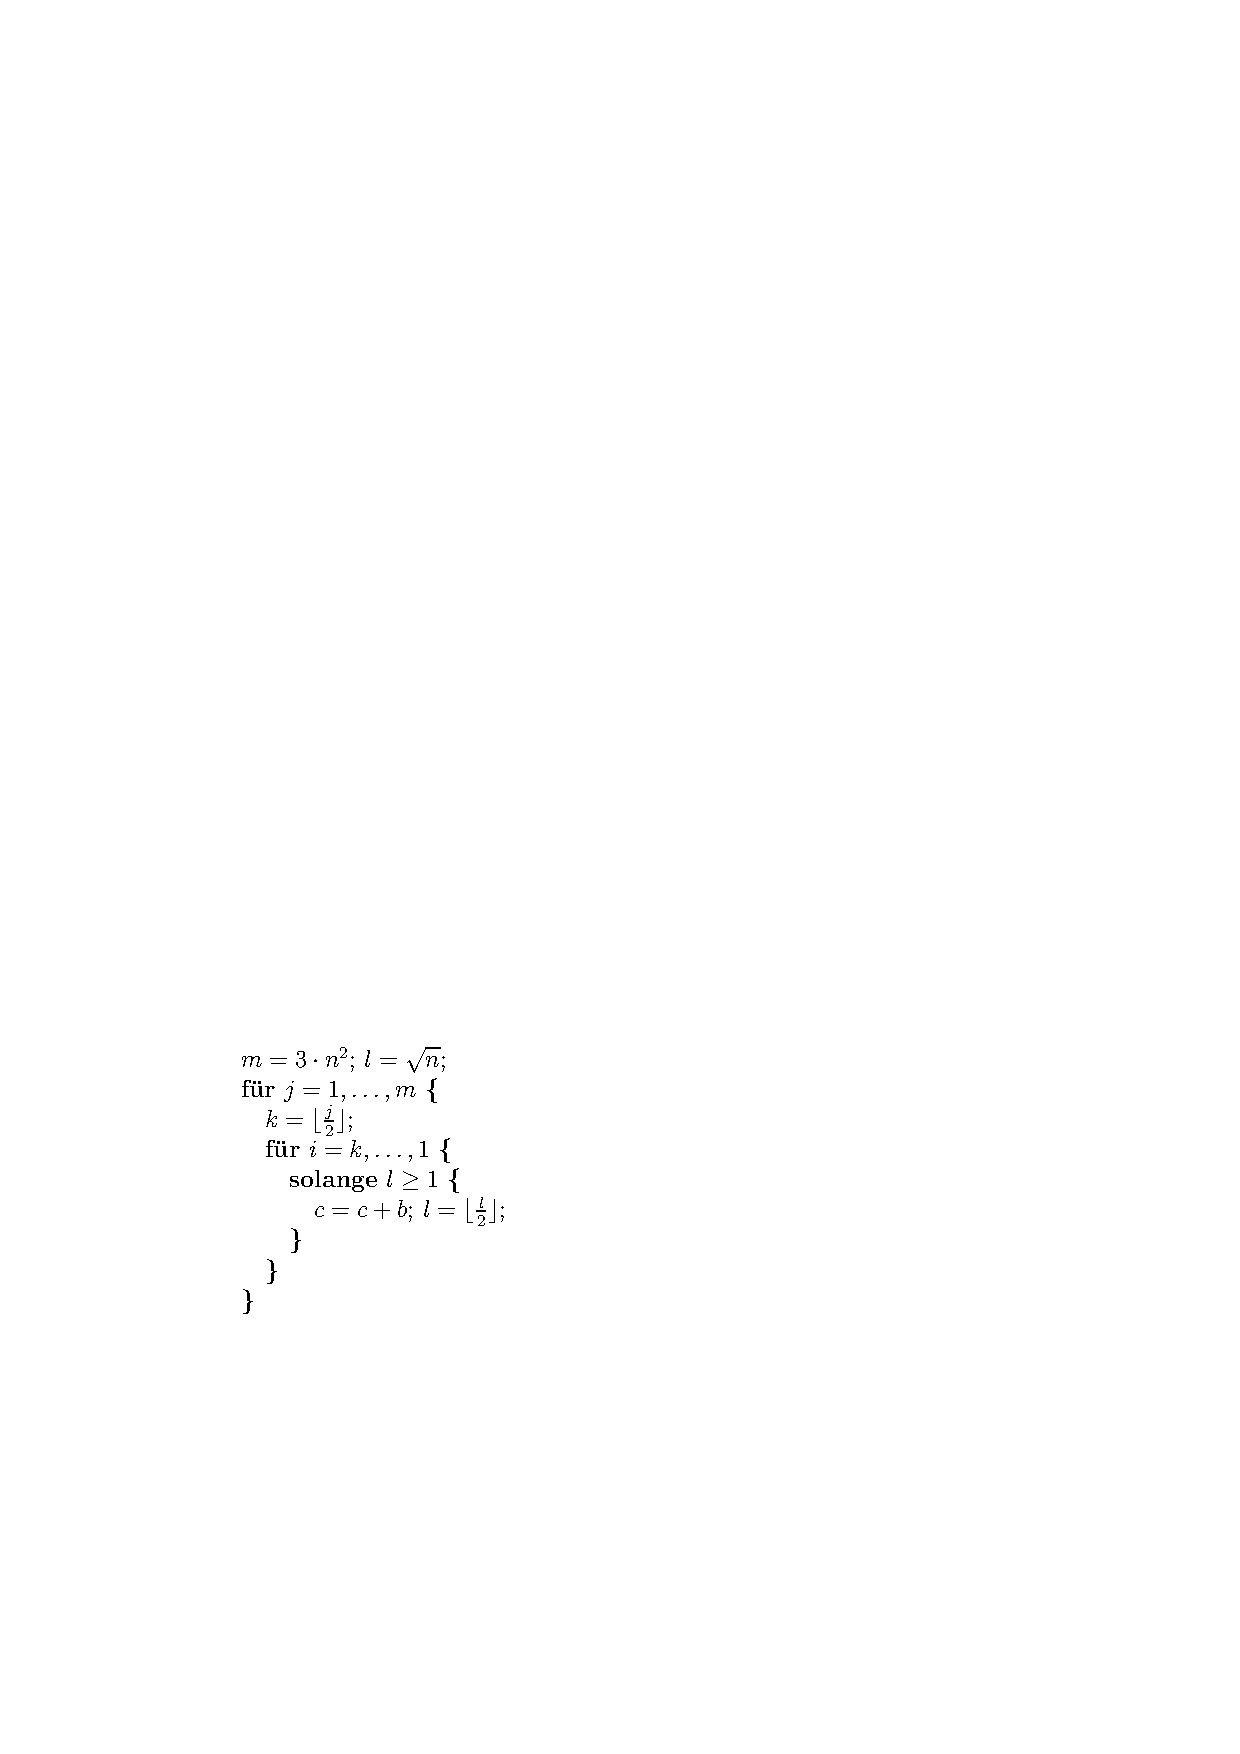
\includegraphics{Figures/Test_2007-11-16_1Ac}
    \label{figure:Test_2007-11-16_1Ac}
\end{minipage}
\begin{minipage}[t]{0.08\textwidth}~\end{minipage}
\begin{minipage}[t]{0.45\textwidth}
    \captionof{figure}{Beispiel 1.c) der Gruppe B}
    \centering
    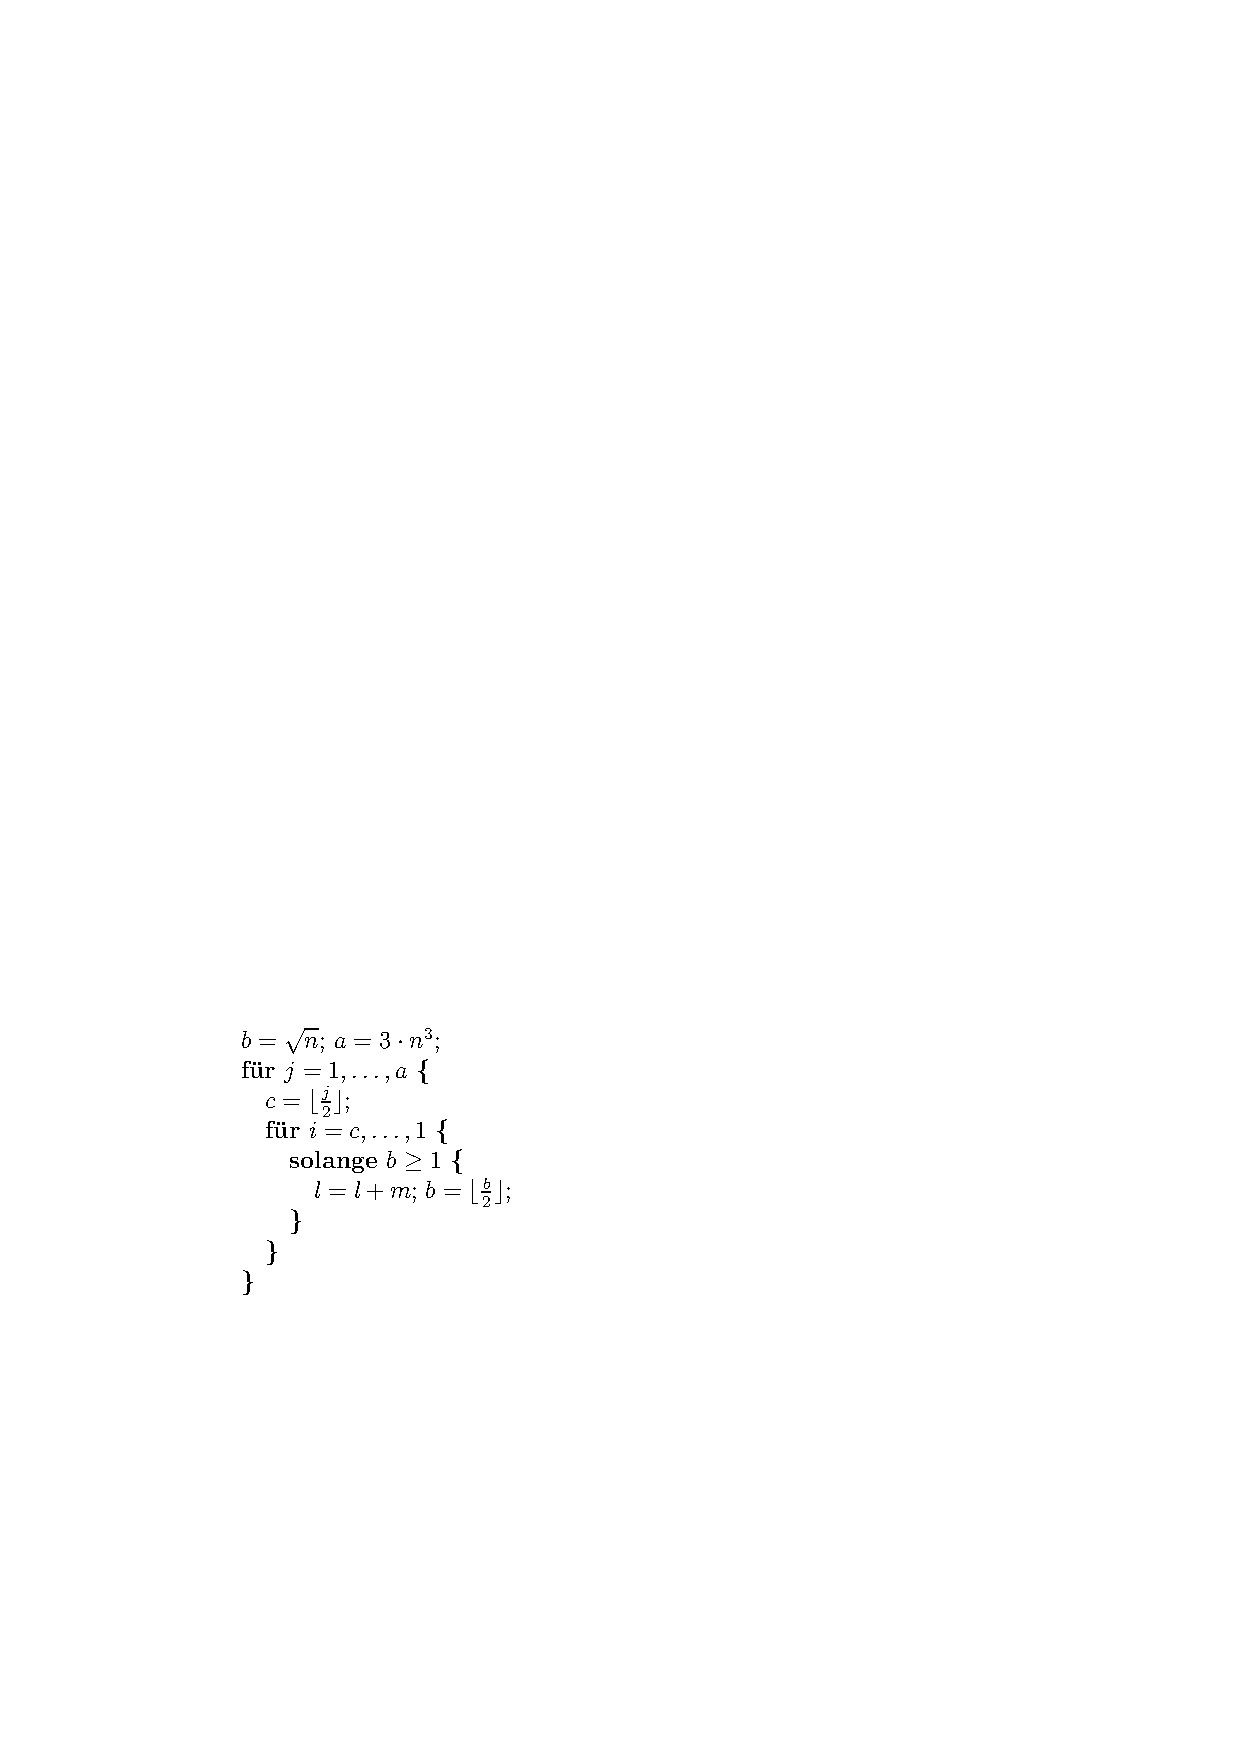
\includegraphics{Figures/Test_2007-11-16_1Bc}
    \label{figure:Test_2007-11-16_1Bc}
\end{minipage}

Die äußerste Schleife läuft von 1 bis $3n²$ und besitzt somit ein
quadratischen Laufzeit. Die zweite für-Schleife läuft jeweils bis zu
$\frac{j}{2}$. Das heißt die Laufzeit beträgt
$\frac{1}{2},\frac{2}{2},\frac{3}{2},\frac{4}{2}\dots\frac{3n²}{2}$. Lassen
wir die Konstante weg ($3n² ⇒ n²$) und ziehen den Term $\frac{1}{2}$ nach
vorne erhalten wir $\frac{1}{2}\left(1,2,3,4\dots n²\right)$. Mit der
Summenformel von Gauß ergibt sich also $\frac{1}{2}⋅(n²+1)⋅\frac{n²}{2}$ und
somit insgesamt eine Laufzeit von $θ\left(n⁴\right)$ für das gesamte
Codestück.\\

Die Analyse des Codes von Abbildung~\ref{figure:Test_2007-11-16_1Bc} führt
analog zu dem vorhergehenden Beispiel auf eine Laufzeit von
$θ\left(n⁶\right)$.

\paragraph{Test vom 25.4.2008}~\\

Wir analysieren den in Abbildung~\ref{figure:Test_2008-04-25_1Ac}
dargestellten Code. Die beiden inneren Schleifen sind abhängig voneinander, da
in der äußeren Schleife $j$ auf ein Drittel verringert wird. Die innere
Schleife läuft also $n,\frac{n}{3},\frac{n}{9},\frac{n}{27}\dots$ mal solange
$j≥1$. Die Summe über diese Terme liegt zwischen n und $2n$. Die inneren
Schleifen ergeben also einen Aufwand von $θ\left(n\right)$.

\begin{minipage}[t]{0.45\textwidth}
    \centering
    \captionof{figure}{Beispiel 1.c) der Gruppe A}
    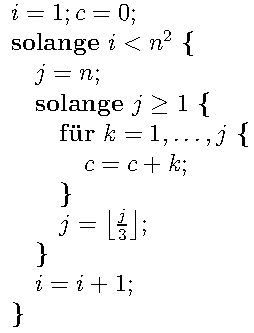
\includegraphics{Figures/Test_2008-04-25_1Ac}
    \label{figure:Test_2008-04-25_1Ac}
\end{minipage}
\begin{minipage}[t]{0.08\textwidth}~\end{minipage}
\begin{minipage}[t]{0.45\textwidth}
    \centering
    \captionof{figure}{Beispiel 1.c) der Gruppe B}
    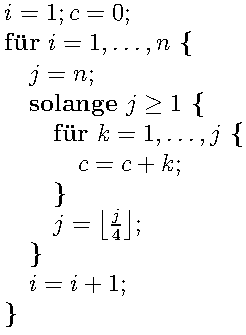
\includegraphics{Figures/Test_2008-04-25_1Bc}
    \label{figure:Test_2008-04-25_1Bc}
\end{minipage}~\\

Die äußere Schleife läuft $n²$ mal. Somit ergibt sich ein Gesamt-Aufwand von
$θ\left(n³\right)$.\\

Nach analoger Analyse zum vorhergehenden Beispiel ergibt sich für den Code von
Abbildung~\ref{figure:Test_2008-04-25_1Bc} eine Laufzeit von
$θ\left(n²\right)$.

\paragraph{Test vom 7.11.2008}~\\

\begin{figure}[htbp]
	\caption{Beispiel 1.c) A der Gruppe A}
	\vskip 0.2cm
	\centering
	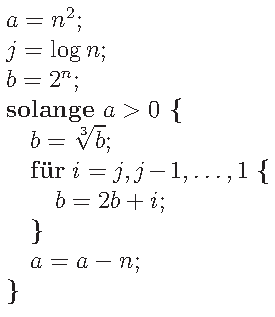
\includegraphics[width=0.32\textwidth]{Figures/Test_2008-11-07_1AcA}
	\label{figure:Test_2008-11-07_1AcA}
\end{figure}

Der zu analysierende Code ist in Abbildung~\ref{figure:Test_2008-11-07_1AcA}
dargestellt. In der äußeren Schleife wird von $a$ immer wieder $n$ abgezogen.
Das können wir $n$ mal machen bis $a≤0$ ist. Die äußere Schleife hat somit
eine Laufzeit in $θ\left(n\right)$. In der inneren Schleife wird von der
Variable $j$, die am Anfang den Wert $log\left(n\right)$ besitzt solange 1
abgezogen bis wir auf einen Wert von 1 kommen. Dieser Schritt kann
$log\left(n\right)$ mal durchgeführt werden. Insgesamt ergibt sich also eine
Laufzeit von $θ\left(log\left(n\right)⋅ n\right)$

\paragraph{Test vom 15.04.2011}~\\

\begin{figure}[htbp]
	\caption{Beispiel 1.a) B der Gruppe A}
	\vskip 0.2cm
	\centering
	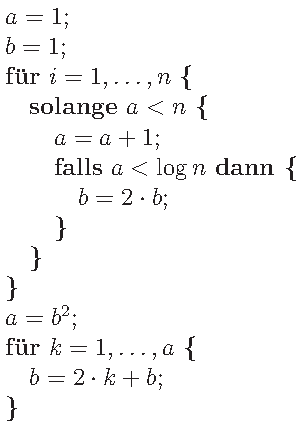
\includegraphics{Figures/Test_2011_04_15_AaB}
	\label{figure:Test_2011_04_15_AaB}
\end{figure}

Der in Abbildung~\ref{figure:Test_2011_04_15_AaB} gezeigte Code soll
analysiert werden. Die äußerste „für”-Schleife wird n mal durchgeführt. Da die
innere „so-lange”-Schleife nur beim ersten dieser n Durchgänge ausgeführt wird
— a wird nachdem es den Wert n erreicht hat nicht mehr auf einen kleineren
Wert gesetzt — kann die Laufzeit der inneren Schleife von $\log(n)$
vernachlässigt werden. Insgesamt ergibt sich für die erste „für”-Schleife also
eine Laufzeit von $θ(n)$. Diese Tatsache kann man auch erkennen wenn man sich
die einzelnen Laufzeiten der äußersten Schleife ansieht:

\begin{itemize}
	\item 1. Durchgang: $θ\left(\log(n) \right)$
	\item 2. Durchgang: $θ(1)$
	\item 3. Durchgang: $θ(1)$
	\item …
	\item n. Durchgang: $θ(1)$
\end{itemize}

Zusammengezählt kommen wir damit auf eine Laufzeit in Theta-Notation von
\[θ\left(\log(n)+\left(n-1\right)⋅ 1\right) \equiv θ\left(n\right)\]

Der Wert von b nach den ersten beiden Schleifen beträgt $2^{\log(n)}$. Dieser
Wert ergibt sich dadurch, dass in der inneren Schleife b $\log(n)$ mal
verdoppelt wurde. Dabei gehen wir hierbei davon aus, das es sich bei $\log(n)$
um den Zweierlogarithmus handelt. Dadurch heben sich der Logarithmus und die
Zweierpotenz (Umkehrfunktion des Zweierlogarithmus) auf und der Wert von $b$
beträgt somit $n$.\\

Der neue Wert der in a gespeichert wird ist also $n²$ ($a=b^2$). Damit kommen
wir für die letzte „für”-Schleife auf eine Laufzeit in Theta-Notation von
$θ(n²)$. Die Gesamtlaufzeit beträgt somit: $$θ\left(n+n²\right) \equiv
θ\left(n²\right)$$

\section{Sortieralgorithmen}

\subsection{Test vom 25.4.2008}

\begin{figure}[htbp]
	\caption{Beispiel 2.c) von Gruppe A}
	\vskip 0.2cm
	\centering
	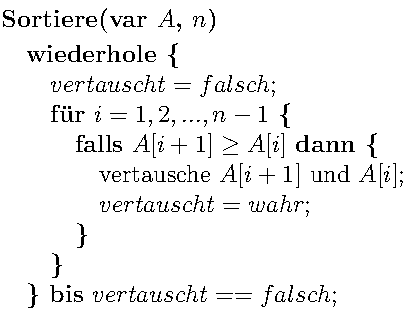
\includegraphics[width=0.5\textwidth]{Figures/Test_2008-04-25_2Ab}
	\label{figure:Test_2008-04-25_2Ab}
\end{figure}

Der in Abbildung~\ref{figure:Test_2008-04-25_2Ab} gezeigte Sortieralgorithmus
wird auf ein Feld $A=\left(A[1],\dots,A[n]\right)$ angewendet. Er sortiert
nicht alle Eingabefolgen korrekt. Wo liegt das Problem und wie kann man es
beheben?\\

Es ist möglich, dass der Algorithmus nicht terminiert. Eine Folge die z.B. zu
einer Endlosschleife führt ist [1,1]. Hier werden als erstes die beiden
Elemente vertauscht da $1≥1$ ist und dann die Variable \texttt{vertauscht} auf
wahr gesetzt. Somit wird die wiederhole-Schleife wieder ausgeführt. In dieser
werden wieder die beiden Elemente vertauscht und \texttt{vertauscht} auf wahr
gesetzt\dots\\

Damit der Algorithmus terminiert muss „$A[i+1] ≥ A[i]$” durch „$A[i+1] >
A[i]$” ersetzt werden.

\section{Hashverfahren}

\subsection{Test vom 25.4.2008}

\begin{figure}[htbp]
	\caption{Beispiel 1.a) von Gruppe B}
	\vskip 0.2cm
	\centering
	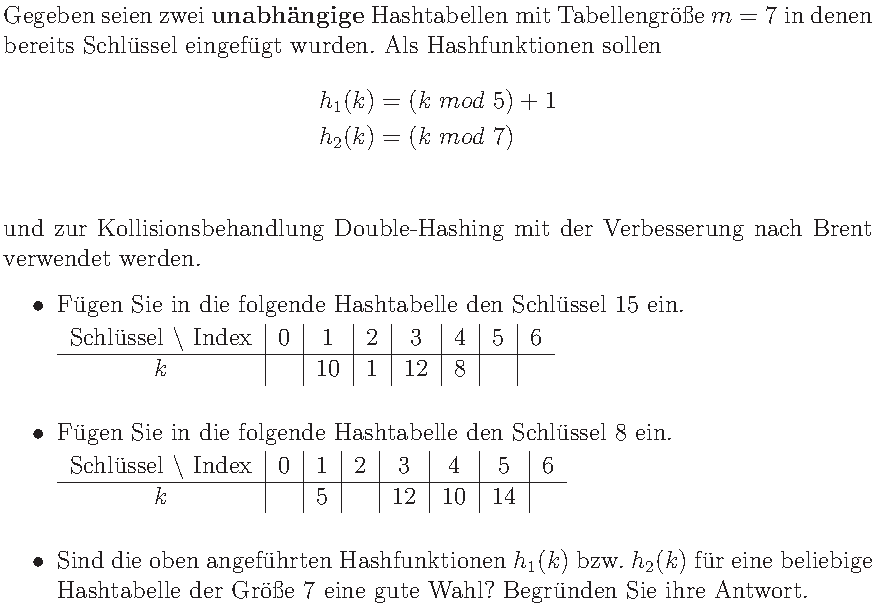
\includegraphics[width=0.9\textwidth]{Figures/Test_2010-01-14_1Ba}
	\label{figure:Test_2010-01-14_1Ba}
\end{figure}

\paragraph{Angabe}

Die Angabe zum Beispiel ist in Abbildung~\ref{figure:Test_2010-01-14_1Ba} zu
sehen.

\paragraph{Lösung}

\begin{align*}
	h\left(k, i\right) &
		= \left( h₁\left(k\right) + i ⋅ h₂\left(k\right) \right) \bmod{m}
	\\
	h\left(k, i \right) &
		= \left(
			\left( k \bmod{5} + 1 \right) + i ⋅ \left(k \bmod{7} \right)
		\right) \bmod{7}
\end{align*}
\begin{align*}
	h\left(15, 0 \right) &
		= \left( 15 \bmod{5} +1 \right) \bmod{7} = \textcolor{orange}{1}
\end{align*}
\begin{align*}
	h\left(15, 1 \right) &
		= \left( \textcolor{orange}{1} + 15 \bmod{7} \right) \bmod{7}
		= \textcolor{aqua}{2}
	\\
	h\left(10, x \right) &
		= \left( \textcolor{orange}{1} + 10 \bmod{7} \right) \bmod{7}
		= 4
\end{align*}
\begin{align*}
	h\left(15, 2 \right) &
		= \left( \textcolor{aqua}{2} + 15 \bmod{7} \right) \bmod{7}
		= \textcolor{violet}{3}
	\\
	h\left(1, x \right) &
		= \left( \textcolor{aqua}{2} + 1 \bmod{7} \right) \bmod{7}
		= 3
\end{align*}
\begin{align*}
	h\left(15, 3 \right) &
		= \left( \textcolor{violet}{3} + 15 \bmod{7} \right) \bmod{7}
		= \textcolor{turquoise}{4}
	\\
	h\left(12, x \right) &
		= \left( \textcolor{violet}{3} + 12 \bmod{7} \right) \bmod{7}
		= 1
\end{align*}
\begin{align*}
	h\left(15, 4 \right) &
		= \left( \textcolor{turquoise}{4} + 15 \bmod{7} \right) \bmod{7}
		= 5
\end{align*}

15 wird an die Stelle 5 gegeben.
\begin{align*}
	h\left(8, 0 \right) &
		= \left( 8 \bmod{5} + 1 \right) \bmod{7}
		= \textcolor{orange}{4}
	\\
	h\left(8, 1 \right) &
		= \left( \textcolor{orange}{4} + 8 \bmod{7} \right) \bmod{7}
		= 5
	\\
	h\left(10, x \right) &
		= \left( \textcolor{orange}{4} + 10 \bmod{7} \right) \bmod{7}
		= 0
\end{align*}

10 wird an Stelle 0 gegeben während 8 an die ursprüngliche Stelle von 10
wandert, also an Stelle 4 eingesetzt wird.\\

Die Hashfunktionen sind keine gute Wahl, da bei $h₂\left(k\right)$ eine
Schrittweite von 0 möglich ist, weiters belegt $h₁\left(k\right)$ niemals
Platz 0 und 6.

\section{Graphen}

\subsection{Test vom 14.1.2011}

\begin{figure}[htbp]
	\caption{Beispiel 3.A vom Test am 14.1.2011}
	\vskip 0.2cm
	\centering
	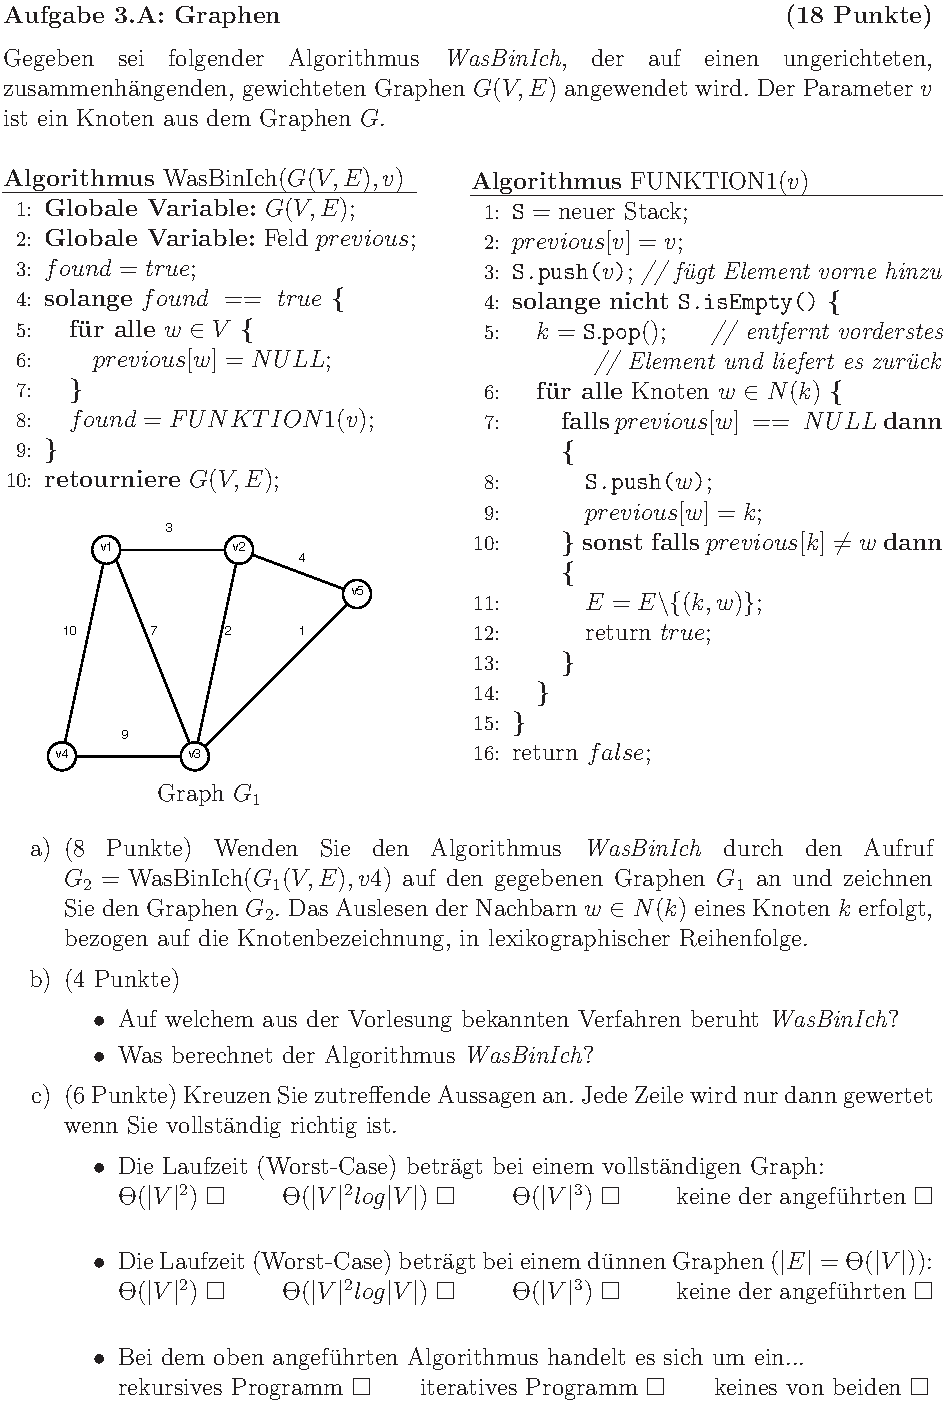
\includegraphics[width=0.95\textwidth]{Figures/Test_2011-01-14_3A}
	\label{figure:Test_2011-01-14_3A}
\end{figure}

\paragraph{a)}

Wir wenden schrittweise den in Abbildung~\ref{figure:Test_2011-01-14_3A}
dargestellten Algorithmus auf den Graphen der ebenfalls in
Abbildung~\ref{figure:Test_2011-01-14_3A} zu sehen ist an und geben jeweils
den Zustand des Graphen und des „previous”-Arrays nach einem Durchlauf von
$FUNKTION1(v_4)$ an.

\subparagraph{1. Schritt}

\begin{center}
	\begin{tabular}{lccccc}
					& v1	& v2	& v3	& v4	& v5\\
		\hline
		previous[v] & NULL	& NULL	& NULL	& NULL	&  NULL
	\end{tabular}
\end{center}

Wir setzen als erstes alle Vorgänger auf den Wert „NULL”. Dann beginnen wir
mit der Ausführung von $FUNKTION1(v4)$ die als erstes den Vorgänger von $v4$
auf sich selbst setzt und dann $v4$ in den Stack gibt. Danach wird $v4$ aus
dem Stack entnommen und all Nachbarknoten von $v4$ der Reihenfolge nach
betrachtet.\\

Der Vorgänger vom ersten Nachbar $v1$ und vom zweiten Nachbar $v3$ werden auf
$v4$ gesetzt. Weiters werden $v1$ und $v3$ der Reihe nach in den Stack $S$
gegeben.\\

\begin{minipage}[b]{0.7\linewidth}
	\begin{center}
		\begin{tabular}{lccccc}
						& v1	& v2	& v3	& v4	& v5\\
			\hline
			previous[v] & v4	& NULL	& v4	& NULL	&  NULL
		\end{tabular}
	\end{center}
\end{minipage}
\begin{minipage}[b]{0.15\linewidth}
	\flushright S:~
\end{minipage}
\begin{minipage}[b]{0.15\linewidth}
	\begin{tabular}{|c|}
		$v3$\\
		$v1$\\
		\hline
	\end{tabular}
\end{minipage}\\

Danach wird $v3$ (=$k$) aus dem Stack entnommen und seine Nachbarn betrachtet.
Da der Vorgänger von $v3$ schon vorher auf $v4$ (=$previous[k]$) gesetzt wurde
und somit nicht $v1$ (=$w$) entspricht wird die Kante $(v3,v1)$ aus dem
Graphen entfernt und die Funktion retourniert den Wert „true”. Damit ergibt
sich nach dem ersten Aufruf von $FUNKTION1(v4)$ folgender Zustand von
„previous”:

\begin{center}
	\begin{tabular}{lccccc}
					& v1	& v2	& v3 & v4	& v5\\
		\hline
		previous[v] & v4	& NULL	& v4 & v4	& NULL\\
	\end{tabular}
\end{center}

Wir erhalten den in Abbildung~\ref{figure:Test_2011-01-14-3A_Step1}
dargestellten Graphen.

\begin{figure}[htbp]
	\caption{Graph nach der ersten Anwendung von $FUNKTION1(v4)$}
	\vskip 0.2cm
	\centering
	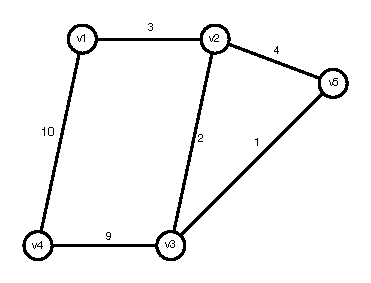
\includegraphics[width=0.5\textwidth]{Figures/Test_2011-01-14-3A_Step1}
	\label{figure:Test_2011-01-14-3A_Step1}
\end{figure}

\subparagraph{2. Schritt}~\\

Nach einer weiteren Anwendung von $FUNKTION1(v4)$ kommen wir auf folgenden
Zustand von „previous”:

\begin{center}
	\begin{tabular}{lccccc}
					& v1	& v2	& v3 & v4	& v5\\
		\hline
		previous[v] & v4	& v3	& v4	& v4 & v3\\
	\end{tabular}
\end{center}

Da es sich beim Vorgänger von $v5$ nicht um $v2$ handelt wird die Kante
$(v5,v2)$ gelöscht und es ergibt sich der in
Abbildung~\ref{figure:Test_2011-01-14-3A_Step2} dargestellte Graph.

\begin{figure}[htbp]
	\caption{Graph nach der zweiten Anwendung von $FUNKTION1(v4)$}
	\vskip 0.2cm
	\centering
	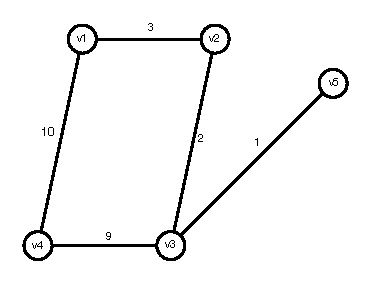
\includegraphics[width=0.5\textwidth]{Figures/Test_2011-01-14-3A_Step2}
	\label{figure:Test_2011-01-14-3A_Step2}
\end{figure}

\subparagraph{3. Schritt}~\\

Nach dem dritten Schritt ergibt sich folgendes „previous”-Array:

\begin{center}
	\begin{tabular}{lccccc}
					& v1	& v2	& v3	& v4	& v5\\
		\hline
		previous[v] & v4	& v3	& v4	& v4	& v3
	\end{tabular}
\end{center}

Nachdem der Vorgänger von $v2$ nicht $v1$ ist wird die Kante $(v2,v1)$
gelöscht und es ergibt sich der Graph von
Abbildung~\ref{figure:Test_2011-01-14-3A_Step3}.

\begin{figure}[htbp]
	\caption{Graph nach der dritten Anwendung von $FUNKTION1(v4)$}
	\vskip 0.2cm
	\centering
	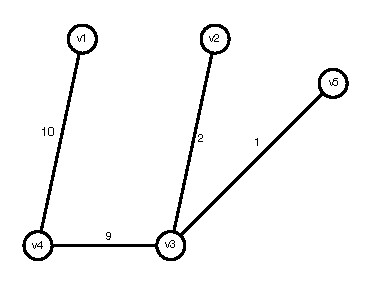
\includegraphics[width=0.5\textwidth]{Figures/Test_2011-01-14-3A_Step3}
	\label{figure:Test_2011-01-14-3A_Step3}
\end{figure}

\subparagraph{4. Schritt}~\\

Nach dem 4. Schritt erhalten wir sowohl das gleiche „previous”-Array als auch
den gleichen Graphen wie im vorigen Schritt. Diesmal wird von der Funktion
allerdings „false” zurückgegeben und der Algorithmus terminiert. Bei $G₂$
handelt es sich also um den in Abbildung~\ref{figure:Test_2011-01-14-3A_Step3}
dargestellten Graphen.

\paragraph{b)}

\begin{itemize}

    \item Der Algorithmus beruht auf dem Tiefensuche-Prinzip (Aus dem Stack
    wird immer der Knoten der als letztes reingegeben wurde als erstes wieder
    entnommen und betrachtet).

    \item „WasBinIch” entfernt die Kreise eines Graphen und bildet somit — bei
    einem zusammenhängenden Graphen — einen (Spann)-Baum.

\end{itemize}

\paragraph{c)}

\begin{itemize}

	\item Die Worst-Case Laufzeit beträgt bei einem vollständigen Graphen
    $θ\left(|V³|\right)$, da der Graph $θ\left(|V|²\right)$ Kanten besitzt die
    Theta $θ\left(|V|\right)$ mal durchgegangen
    werden~\cite{Juggl3r_Beispiel3}.

    \item Die Worst-Case Laufzeit beträgt bei einem dünnen Graphen
    $θ\left(|V²|\right)$, da der Graph $θ\left(|V|\right)$ Kanten besitzt die
    Theta $θ\left(|V|\right)$ mal durchgegangen
    werden~\cite{Juggl3r_Beispiel3}.

    \item Bei dem Algorithmus handelt es sich um ein iteratives Programm.

\end{itemize}

\section{Beispiel für dynamische Programmierung}

\subsection{Angabe}

Mit $40℃$ im Schatten hat sich der Sommer gerade eingestellt. Da dir
heiß ist, möchtest du die hohe Temperatur mit dem Verzehr eines großen Eises
für dich etwas erträglicher gestalten. Als Student verfügst du nur über ein
begrenztes Einkommen und beschließt daher maximal sieben Euro auszugeben. Die
Eisreserven sind gerade knapp und deswegen darfst von jeder Sorte nur eine
Kugel nehmen. Um zu bestimmen welche Sorten die bestmögliche Kombination unter
den gegebenen Bedingungen darstellen, beschließt du dynamische Programmierung
zu verwenden.

\begin{table}[H]
	\begin{center}
		\begin{tabular}{lcc}
			Eissorte & Genussfaktor & Kosten\\
			\hline
			Creme de la Creme	& 10	& 3\\
			Brokkoli			& 3		& 1\\
			Vanille				& 7		& 2\\
			Málaga				& 8		& 2\\
			Schokolade			& 7		& 3\\
			Kaviar				& 6		& 8\\
		\end{tabular}
	\end{center}
\caption{Eissorten}
\label{table:Label}
\end{table}

\subsection{Erstellen der Matrix}

Als erstes erstellen wir eine Tabelle mit den nötigen Einträgen. Da wir die
Wahl zwischen sechs verschiedenen Sorten haben, sollte unsere Matrix
eigentlich sieben Zeilen besitzen (eine zusätzliche Zeile für die Wahl keiner
einzigen Sorte). Die Sorte Kaviar überschreitet allerdings unsere bescheidenen
Mittel von sieben Euro. Deshalb brauchen wir diese nicht zu beachten und somit
können wir auf die Zeile für diese Sorte komplett verzichten. Somit erstellen
wir eine Tabelle mit insgesamt 6 Zeilen (Tabelle \ref{table:Leer}).

\begin{table}[H]
	\begin{center}
		\begin{tabular}{l|cccccccc}
			$⇓$Eissorte $⇒$ Kosten & 0 & 1 & 2 & 3 & 4 & 5 &
			6 & 7\\
			\hline
			Keine Sorte			&	&	&	&	&	&	&	&\\
			Creme de la Creme	&	&	&	&	&	&	&	&\\
			Brokkoli			&	&	&	&	&	&	&	&\\
			Vanille				&	&	&	&	&	&	&	&\\
			Málaga				&	&	&	&	&	&	&	&\\
			Schokolade			&	&	&	&	&	&	&	&\\
		\end{tabular}
	\end{center}
\caption{Matrix für unser Beispiel}
\label{table:Leer}
\end{table}

Wie wir sehen stehen die Spalten für die Kosten (Gewicht) des Eis und die
Zeilen für die verschiedenen Eissorten (Gegenstände). In den Zellen der
Tabelle tragen wir den Genussfaktor (Wert) ein.

\begin{leftbar}
	\textbf{Anmerkung:}\\

	Üblicherweise werden in der LVA „Algorithmen und Datenstrukturen 1”,
    Koffer oder Rucksäcke so gepackt, dass ein bestimmtes Gewicht nicht
    überschritten wird und sich gleichzeitig ein möglichst hoher Spaßfaktor
    ergibt.\\

	In diesem Zusammenhang wird der Wert der maximiert werden soll auch
    manchmal als Kosten oder „c” bezeichnet. In diesem Musterbeispiel stellen
    die Kosten des Eises allerdings das eigentliche Gewicht „w”, also die
    Randbedingung die nicht überschritten werden soll dar. Dahingegen wird die
    Variable die maximiert werden soll hier als Genussfaktor bezeichnet, sie
    stellt also laut LVA-Regelung das eigentliche „c” dar.\\

	Ich hoffe mal diese Erläuterung verwirrt nicht mehr als sie hilft.\\

	\textbf{Kurzfassung:}\\
	w\dots Kosten des Eises\\
	c\dots Genussfaktor
\end{leftbar}

Es ist leicht feststellbar, dass wenn wir keine einzige Sorte Eis auswählen
wir davon auch keinen Nutzen haben. Somit können wir die erste Spalte mit
lauter Nullen füllen. Da es leider kein „Gratis-Eis” gibt können wir auch
keine Sorte wählen ohne zumindest etwas zu zahlen. Daraus resultiert, dass
auch die Spalte mit Kosten Null mit lauter Nullen gefüllt werden muss.
Insgesamt ergibt sich also das in Tabelle \ref{table:Initialisierung}
dargestellte Bild.

\begin{table}[H]
	\begin{center}
		\begin{tabular}{l|cccccccc}
			$⇓$Eissorte $⇒$ Kosten & 0 & 1 & 2 & 3 & 4 & 5 &
			6 & 7\\
			\hline
			Keine Sorte			& 0 & 0 & 0 & 0 & 0 & 0 & 0 & 0 \\
			Creme de la Creme	& 0 &	&	&	&	&	&	&	\\
			Brokkoli			& 0 &	&	&	&	&	&	&	\\
			Vanille				& 0 &	&	&	&	&	&	&	\\
			Málaga				& 0 &	&	&	&	&	&	&	\\
			Schokolade			& 0 &	&	&	&	&	&	&	\\
		\end{tabular}
	\end{center}
\caption{Initialisierung der Matrix}
\label{table:Initialisierung}
\end{table}

Nach diesem Schritt könne wir endlich anfangen die erste Eissorte zu
betrachten. „Creme de la Creme” besitzt einen Genussfaktor von 10 und Kosten
von 3. Wir tragen also in der ersten Zeile bei Kosten 3 einen Genussfaktor von
10 ein (Tabelle \ref{table:1_Eis}).

\begin{table}[H]
	\begin{center}
		\begin{tabular}{l|cccccccc}
			$⇓$Eissorte $⇒$ Kosten & 0 & 1 & 2 & 3 & 4 & 5 &
			6 & 7\\
			\hline
			Keine Sorte			& 0 & 0 & 0 & 0	 & 0	& 0 & 0 & 0 \\
			Creme de la Creme	& 0 &	&	& 10 &	&	&	&	\\
			Brokkoli			& 0 &	&	&	 &	&	&	&	\\
			Vanille				& 0 &	&	&	 &	&	&	&	\\
			Málaga				& 0 &	&	&	 &	&	&	&	\\
			Schokolade			& 0 &	&	&	 &	&	&	&	\\
		\end{tabular}
	\end{center}
\caption{Matrix nach der Betrachtung der ersten Eissorte}
\label{table:1_Eis}
\end{table}

Nun sehen wir uns die Eissorte „Brokkoli” an, die nur einen geringen
Genussfaktor von 3 besitzt, dafür aber auch nur einen Euro kostet. Da in der
Spalte mit Kosten 1 in der vorhergehenden Zeile noch kein Wert steht, können
wir in diese Spalte den Genussfaktor dieses Eises eintragen.\\

Von der vorhergehenden Zeile sehen wir, dass wir schon die Möglichkeit
besitzen ein Eis zu wählen das die Kosten 3 und Genussfaktor 10 besitzt.
Dieses können wir natürlich weiterhin auswählen. Deshalb übertragen wir den
Wert von der oberen Zeile in Spalte 3.\\

Weiters können wir jetzt die Eissorte von vorher nehmen und mit der aktuellen
Sorte, Brokkoli kombinieren. Insgesamt ergeben sich dadurch Kosten von 4 und
ein Genusswert von 13 den wir in die aktuelle Zeile eintragen. Nach diesen
Überlegungen erhalten wir die in Tabelle \ref{table:2_Eis} dargestellte Matrix.

\begin{table}[H]
	\begin{center}
		\begin{tabular}{l|cccccccc}
			$⇓$Eissorte $⇒$ Kosten & 0 & 1 & 2 & 3 & 4 & 5 &
			6 & 7\\
			\hline
			Keine Sorte			& 0 & 0 & 0 & 0	 &	0 & 0	& 0 & 0 \\
			Creme de la Creme	& 0 &	&	& 10 &	  & &	&	\\
			Brokkoli			& 0 & 3 &	& 10 & 13 & &	&	\\
			Vanille				& 0 &	&	&	 &	  & &	&	\\
			Málaga				& 0 &	&	&	 &	  & &	&	\\
			Schokolade			& 0 &	&	&	 &	  & &	&	\\
		\end{tabular}
	\end{center}
\caption{Matrix nach der Betrachtung der zweiten Eissorte}
\label{table:2_Eis}
\end{table}

Die Geschmackssorte Vanille besitzt einen Genussfaktor von 7 bei Kosten von 2
Euro. Da bei der Spalte mit Kosten 2 noch kein Wert eingetragen ist schreiben
wir dort den Genussfaktor von der aktuellen Eissorte Vanille an.\\

Jetzt betrachten wir wieder die Zeile davor um zu sehen welche weiteren
Kombinationen möglich sind. Wenn wir Vanille-Eis und den ersten Wert in der
oberen Zeile wählen kommen wir auf Kosten von 3 und einen Genussfaktor von 10.
Dieser Wert entspricht dem von der vorhergehenden Zeile. Wir haben also eine
Kombination gefunden die gleich gut wie die vorhergehende war. Im Endeffekt
bleibt der Wert in der Spalte 3 also der Selbe.\\

In Spalte 3 der vorhergehenden Zeile befindet sich der Genussfaktor 10.
Zusammen mit der aktuellen Sorte ergibt sich ein Genussfaktor von 17 bei
Kosten von 5 Euro. Da sich in der Spalte 5 noch kein Wert befindet tragen wir
diesen Genussfaktor also dort ein.\\

Zum Schluss betrachten wir noch den Genussfaktor von 13 bei Kosten von 4.
Zusammen mit der aktuellen Eissorte ergibt sich ein Genussfaktor von 20 bei
Kosten von 6. Wir tragen also diesen Wert ein. Die anderen Werte werden von
oben übernommen, da wir noch keine besseren Kombinationen für die Kosten von 1
und 4 gefunden haben (Tabelle \ref{table:3_Eis}).

\begin{table}[H]
	\begin{center}
		\begin{tabular}{l|cccccccc}
			$⇓$Eissorte $⇒$ Kosten & 0 & 1 & 2 & 3 & 4 & 5 &
			6 & 7\\
			\hline
			Keine Sorte			& 0 & 0 & 0 & 0	 &	0 &	 0 & 0 & 0	\\
			Creme de la Creme	& 0 &	&	& 10 &	  &	   &	&	\\
			Brokkoli			& 0 & 3 &	& 10 & 13 &	   &	&	\\
			Vanille				& 0 & 3 & 7 & 10 & 13 & 17 & 20 &	\\
			Málaga				& 0 &	&	&	 &	  &	   &	&	\\
			Schokolade			& 0 &	&	&	 &	  &	   &	&	\\
		\end{tabular}
	\end{center}
\caption{Matrix nach der Betrachtung der dritten Eissorte}
\label{table:3_Eis}
\end{table}

„Málaga” besitzt einen Genussfaktor von 8 bei Kosten von 2 Euro. Da der
Genusswert höher als der bisher gefundene von 7 ist schreiben wir diesen in
die dafür vorgesehene Spalte.\\

Bei den Kosten von 1 übernehmen wir wieder den Wert von oben, da mit der
aktuellen Eissorte natürlich keine Kombination möglich ist die Kosten von 1
aufweist.\\

Weiters tragen wir in Spalte 3 einen Genusswert von 11 ein, der sich aus dem
Genusswert 3 aus der ersten Spalte der letzten Zeile und dem Genusswert von
Málaga ergibt.\\

Wir betrachten den nächsten Wert von 7 bei Kosten von 2 aus der vorhergehenden
Zeile. Eine Kombination mit Málaga gibt einen Genussfaktor von 15 bei Kosten
von 4. Dieser Wert ist höher als der Vorhergehende in Spalte 4 und wird
deshalb dort eingetragen.\\

Der nächste Genussfaktor aus der vorhergehenden Zeile ist 10. Gemeinsam mit
der aktuellen Sorte kommt man also auf einen Genussfaktor von 18 bei einem
Gewicht von fünf. Dieser wird da er größer als 17 ist, in die fünfte Spalte
eingetragen.\\

13, der nächste Genusswert, ergibt zusammen mit dem aktuellen Eis einen Wert
von 21 und wird deshalb in Spalte 6 (=4+2) eingetragen.\\

Genussfaktor 17 kombiniert mit dem Genussfaktor von Málaga-Eis ergibt den Wert
von 25 der auf Grund der Kosten von 7 Euro in die korrespondierende Spalte
geschrieben wird.\\

Da der letzte Wert aus der vorhergehenden Zeile schon Kosten von 6 besitzt und
diese zusammen mit den Kosten des aktuellen Eises über die festgesetzten
Maximalkosten von 7 Euro hinausgeht brauchen wir diesen nicht mehr zu
betrachten und kommen schließlich auf Tabelle \ref{table:4_Eis}.

\begin{table}[H]
	\begin{center}
		\begin{tabular}{l|cccccccc}
			$⇓$Eissorte $⇒$ Kosten & 0 & 1 & 2 & 3 & 4 & 5 &
			6 & 7\\
			\hline
			Keine Sorte			& 0 & 0 & 0 & 0	 &	0 &	 0 & 0 & 0	 \\
			Creme de la Creme	& 0 &	&	& 10 &	  &	   &	&	 \\
			Brokkoli			& 0 & 3 &	& 10 & 13 &	   &	&	 \\
			Vanille				& 0 & 3 & 7 & 10 & 13 & 17 & 20 &	 \\
			Málaga				& 0 & 3 & 8 & 11 & 15 & 18 & 21 & 25 \\
			Schokolade			& 0 &	&	&	 &	  &	   &	&	 \\
		\end{tabular}
	\end{center}
\caption{Matrix nach der Betrachtung der vierten Eissorte}
\label{table:4_Eis}
\end{table}

Nach der gleichen Vorgehensweise wie in den Schritten zuvor kommen wir,
nachdem wir auch die letzte Eissorte betrachtet haben auf die in Tabelle
\ref{table:5_Eis} dargestellte Matrix.

\begin{table}[H]
	\begin{center}
		\begin{tabular}{l|cccccccc}
			$⇓$Eissorte $⇒$ Kosten & 0 & 1 & 2 & 3 & 4 & 5 &
				6 & 7\\
			\hline
			Keine Sorte			& \textcolor{orange}{0} & 0 & 0 & 0	& 0 & 0 &
				0 & 0\\
			\textbf{Creme de la Creme} & 0 & & & \textcolor{orange}{10} & & &
				&\\
			Brokkoli			& 0 & 3 & & \textcolor{orange}{10} & 13 & &
				&\\
			\textbf{Vanille}	& 0 & 3 & 7 & 10 & 13 & \textcolor{orange}{17} &
				20 &\\
			\textbf{Málaga}		& 0 & 3 & 8 & 11 & 15 & 18 & 21
				& \textcolor{orange}{25}\\
			Schokolade			& 0 & 3 & 8 & 11 & 15 & 18 & 21
				& \textcolor{orange}{\emph{25}}\\
		\end{tabular}
	\end{center}
\caption{Matrix nach der Betrachtung der fünften Eissorte}
\label{table:5_Eis}
\end{table}

\subsection{Rückverfolgung}

Wenn wir die letzte Zeile von Tabelle \ref{table:5_Eis} betrachten, sehen wir
das wir einen maximalen Genussfaktor von 25 erhalten. Um nun zurückzurechnen
welche Auswahl uns zu diesem Wert geführt haben gehen wir die Tabelle
rückwärts durch.\\

Wir starten bei Wert 25 in der letzten Zeile. Da es sich beim Genussfaktor in
der darüberliegenden Zeile in derselben Spalte um den gleichen Wert handelt
schließen wir daraus, dass wir die Sorte Schokolade nicht ausgewählt haben.\\

Wenn wir nach dem ersten Vorkommen des Wertes 25 in der Spalte mit Kosten 7
suchen landen wir in der vorletzten Zeile und sehen, dass die Sorte
\emph{Málaga} ausgewählt wurde. Wir ziehen also vom gesamten Genussfaktor den
Genussfaktor dieser Sorte ab. Somit kommen wir auf einen Wert von 17. Diesen
Wert müssen wir in der Spalte 5 suchen, da von den Gesamtkosten von 7 die
Kosten des Málaga-Eises von 2 abgezogen werden.\\

Wir suchen die Tabellenzeilen in Spalte 5 nach dem ersten Auftreten des
Genussfaktor 17 ab und werden in der Zeile mit der Sorte \emph{Vanille}
fündig. Wir haben also auch diese Eissorte ausgewählt. Wiederum ziehen wir den
Genussfaktor dieses Eises vom dem übrig gebliebenen Genussfaktor 17 ab und
bekommen den Wert 10. Als neue Kosten erhalten wir den Wert 3 (=5-2).\\

Der Genussfaktor von 10 tritt erstmals in der Zeile der Eissorte \emph{„Creme
de la Creme”} auf, die also auch gewählt wurde. Da diese Sorte einen
Genussfaktor von 10 besitzt ergibt sich bei weiterer Subtraktion vom vorher
übrig gebliebenen Genussfaktor ein Wert von Null. Es wurde also keine weitere
Sorte gewählt.\\

Eine Plausibilitätsüberprüfung der gesamten Werte ist in Gleichung
\ref{equation:Kosten} und \ref{equation:Wert} zu sehen. Sie ergibt die
erwarteten Werte und lässt so zumindest darauf hoffen, dass wir die optimale
Lösung, unter der gegebenen Einschränkung nicht mehr als sieben Euro
auszugeben, gefunden haben.

\begin{equation}
	\label{equation:Kosten}
	w_{gesamt} = w_{Malaga} + w_{Vanille} + w_{Creme\_de\_la\_Creme} = \
	2 + 2 + 3 = 7
\end{equation}

\begin{equation}
	\label{equation:Wert}
	c_{gesamt} = c_{Malaga} + c_{Vanille} + c_{Creme\_de\_la\_Creme} = \
	8 + 7 + 10 = 25
\end{equation}

\subsection{Vollständiges Ausfüllen der Tabelle}

Tabelle \ref{table:5_Eis} stellt alle möglichen Lösungen eigentlich schon dar
und sollte auch beim Test durchaus als richtig gewertet werden. Um eine meiner
Meinung nach nur verwirrendere „vollständige” Darstellung nach der gegebenen
Formel zu erhalten muss man die vorhergehende Tabelle noch leicht verändern.\\

So sind die fehlenden Werte jeweils durch den größtmöglichen Wert den sich
durch die vorhergehende Zeile oder Spalte ergeben zu ersetzen. Auch schon
ausgefüllte Werte müssen durch eventuell auftretende größere Werte, die sich
in vorhergehenden Zeilen oder Spalten ergeben haben können, ersetzt werden.\\

Die „vollständige” Matrix für das vorhergehende Beispiel wird in Tabelle
\ref{table:Vollstaendig} gezeigt. Zu beachten ist, dass diese Matrix wie
leicht nachzuvollziehen ist auch „nicht sinnvolle” Werte enthält.

\begin{table}[H]
	\begin{center}
		\begin{tabular}{c|cccccccc}
			$⇓$Eissorte $⇒$ Kosten & 0 & 1 & 2 & 3 & 4 & 5 &
			6 & 7\\
			\hline
			Keine Sorte			& 0 & 0 & 0 & 0	 &	0 &	 0 & 0 & 0	 \\
			Creme de la Creme	& 0 & 0 & 0 & 10 & 10 & 10 & 10 & 10 \\
			Brokkoli			& 0 & 3 & 3 & 10 & 13 & 13 & 13 & 13 \\
			Vanille				& 0 & 3 & 7 & 10 & 13 & 17 & 20 & 20 \\
			Málaga				& 0 & 3 & 8 & 11 & 15 & 18 & 21 & 25 \\
			Schokolade			& 0 & 3 & 8 & 11 & 15 & 18 & 21 & 25 \\
		\end{tabular}
	\end{center}
\caption{„Vollständige” Tabelle}
\label{table:Vollstaendig}
\end{table}

\section{Uni Wien}

\subsection{Test vom 3.10.2011}

\paragraph{Aufgabe 1}

\subparagraph{a)} Geben Sie ein Programm in C++ artigem Pseudocode an, dessen
Aufwand von der Ordnung $Ω(n)$ und $O(n²)$, aber nicht von der Ordnung $Θ(n)$
oder $Θ(n²)$ ist.

\begin{leftbar}
	\input{Code/Aufgabe1a_2011_10_03}
\end{leftbar}

Aufwand: $Θ\left(n·\log\left(n\right)\right)$

\subparagraph{b)}

Geben Sie in C++ artigem Pseudocode eine rekursive Funktion an, deren
Laufzeitordnung $Θ\left( n⁴ \log \left( n \right) \right)$ ist. Zeigen Sie mit
Hilfe des Mastertheorems, dass Ihre Funktion wirklich die geforderte
Laufzeitordnung hat.

\begin{leftbar}
	\input{Code/Aufgabe1b_2011_10_03}
\end{leftbar}

Da $\log_b (a) = c$ ergibt sich eine Laufzeit $T(n) = n^c \log n = n^4 \log n$.

\paragraph{Aufgabe 2}

Addieren Sie zu Ihrer Matrikelnummer die Zahl 573296148. Die Ziffern der Summe
seien in der Reihenfolge von links nach rechts in einem Array gespeichert.
Sortieren Sie die Ziffern aufsteigend mit

\begin{enumerate}[a.]
	\item Counting Sort.
	\item Quicksort.
	\item Selection Sort.
\end{enumerate}

Geben Sie jeweils alle benötigten Zwischenschritte so genau an, dass der
Ablauf des Algorithmus klar ersichtlich wird.

\subparagraph{a)}

$ Matrikelnummer + 573 296 148 = 1 234 567 + 573 296 148 =  574 530 715 $\\

Zu sortierendes Array (A):
\begin{center}
	\newcommand{\columnWidth}{0.5cm}
	\begin{tabular}{|p{\columnWidth}|p{\columnWidth}|p{\columnWidth}
					|p{\columnWidth}|p{\columnWidth}|p{\columnWidth}
					|p{\columnWidth}|p{\columnWidth}|p{\columnWidth}|}
		\hline
		5 & 7 & 4 & 5 & 3 & 0 & 7 & 1 & 5\\
		\hline
	\end{tabular}
\end{center}

Zählerarray (C):

\begin{center}
	\newcommand{\columnWidth}{0.5cm}
	\begin{tabular}{|p{\columnWidth}|p{\columnWidth}|p{\columnWidth}
					|p{\columnWidth}|p{\columnWidth}|p{\columnWidth}
					|p{\columnWidth}|p{\columnWidth}|p{\columnWidth}|
					p{\columnWidth}|}
		\hline
		0 & 1 & 2 & 3 & 4 & 5 & 6 & 7 & 8 & 9\\
		\hline
		\hline
		0 & 0 & 0 & 0 & 0 & 0 & 0 & 0 & 0 & 0\\
		1 & 1 & 0 & 1 & 1 & 3 & 0 & 2 & 0 & 0\\
		1 & 2 & 2 & 3 & 4 & 7 & 7 & 9 & 9 & 9\\
		\hline
	\end{tabular}
\end{center}

Sortiertes Array (B):

\begin{center}
	\newcommand{\columnWidth}{0.5cm}
	\begin{tabular}{|p{\columnWidth}|p{\columnWidth}|p{\columnWidth}
					|p{\columnWidth}|p{\columnWidth}|p{\columnWidth}
					|p{\columnWidth}|p{\columnWidth}|p{\columnWidth}|}
		\hline
		 1 & 2 & 3 & 4 & 5 & 6 & 7 & 8 & 9 \\
		\hline
		   &   &   &   &   &   & 5 &   &   \\
		   & 1 &   &   &   &   & 5 &   &   \\
		   & 1 &   &   &   &   & 5 & 7 &   \\
		 0 & 1 &   &   &   &   & 5 & 7 &   \\
		 0 & 1 & 3 &   &   &   & 5 & 7 &   \\
		 0 & 1 & 3 &   &   & 5 & 5 & 7 &   \\
		 0 & 1 & 3 & 4 &   & 5 & 5 & 7 &   \\
		 0 & 1 & 3 & 4 &   & 5 & 5 & 7 & 7 \\
		 0 & 1 & 3 & 4 & 5 & 5 & 5 & 7 & 7 \\
		\hline
	\end{tabular}
\end{center}


%-- Bibliography --------------------------------------------------------------

\titleformat{\section}{\sffamily\bfseries}{}{0pt}{}[{\color{aqua}\hrule}]

\printbibliography

\end{document}
